% \begin{savequote}[8cm]
% Alles Gescheite ist schon gedacht worden.\\
% Man muss nur versuchen, es noch einmal zu denken.

% All intelligent thoughts have already been thought;\\
% what is necessary is only to try to think them again.
%   \qauthor{--- Johann Wolfgang von Goethe \cite{von_goethe_wilhelm_1829}}
% \end{savequote}

\chapter{\label{ch:2-background}Background}

    \minitoc

    \todo{Introduce that going to introduce notation and give the building blocks this thesis builds off}

    \todo{comment about notation like charlies, $\one$ for example. Also trends of notation that we use: $\tilde{V}$ is (neural net) function approx, $\bar{V}$ is sample average, $\hat{V}$ is estimating something, $\bff{V}$ is a vector, $\cl{V}$ is a set, and these notations can be combined, $\bfcl{V}$ is a set of vectors, typeface text $\texttt{V}$ typically refers to things that are more implementation details}







    


\section{Markov Decision Processes}
\label{sec:2-1-mdps}

    \hide{\todo{chatgpt the intro stuff}}

    In this section \textit{Markov Decision Processes} (MDPs) are introduced, along with related defintions of \textit{policies} and \textit{trajectories}. MDPs give a mathematical framework for problems concerning sequential decision making under uncertainty, and in this thesis will be the framework used to model the environment that agents act in. An MDP contains, among other things, a set of states and actions. States are sampled according to a transition distribution which depends on the current state and current action being taken (the Markov assumption). Any time an action is taken from a state the agent recieves an instantaneous reward, according to a reward function that depends on the state and action taken.

    This thesis is concerned with discrete, finite, fully-observable and finite-horizon Markov Decision Processes, meaning that the state and action spaces are discrete and finite, and any \textit{trajectories} (sequences of states, actions and rewards) are of a finite length. 

    \begin{defn}
        \label{def:mdp}
        A \textnormal{Markov Decision Process} (MDP) is a tuple $\cl{M}=(\cl{S},s_0,\cl{A},R,p,H)$, where $\cl{S}$ is a set of states, $s_0\in\cl{S}$ is an initial state, $\cl{A}$ is a set of actions, $R(s,a)$ is a reward function $\cl{S}\times \cl{A}\rightarrow \bb{R}$, $p(s' | s,a)$ is a next state transition distribution $\cl{S} \times \cl{A} \times \cl{S} \rightarrow [0,1]$ and $H\in\bb{N}$ is a finite-horizon time bound. \todo{I would quite like to make this indefinite horizon. Then also thts would specify a planning horizon H, and heuristic function not unecessary for mctsmode being false}
    \end{defn}

    \begin{figure}
        \centering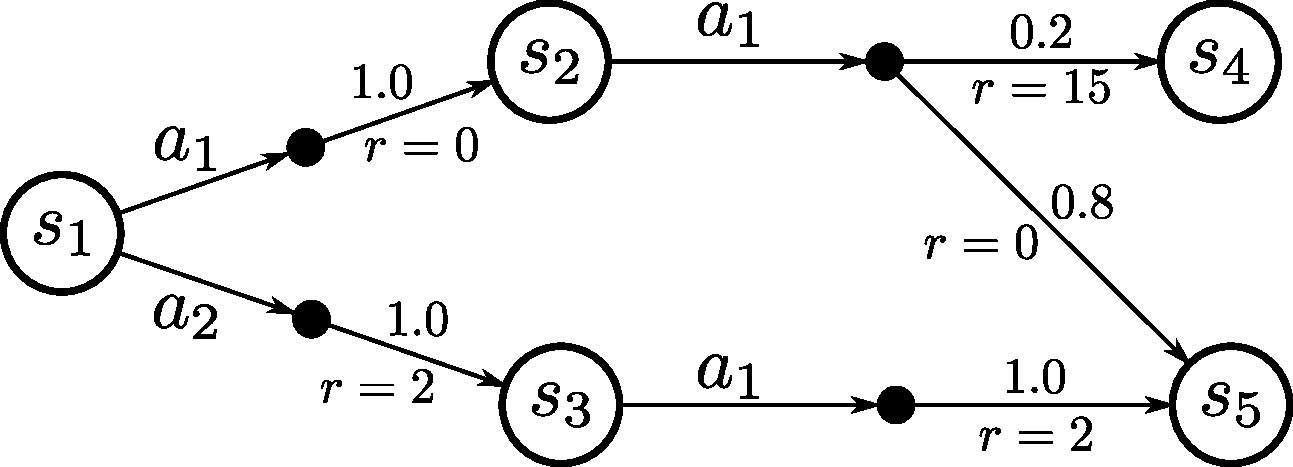
\includegraphics[width=0.8\textwidth]{figures/ch2/example_mdp.pdf} 
        \caption[An example MDP $\cl{M}$.]{An example MDP $\cl{M}$, where \todo{description of MDP drawn}}
        \label{fig:mdp_eg}
    \end{figure}

    An example MDP is shown in Figure \ref{fig:mdp_eg}. Notationally, it is convenient to define the set of successor states, that is the set of states that could be reached after taking an action from the current state of the MDP:
    \begin{defn}
        \label{def:succ}
        The set of \textnormal{successor states} $\suc{s}{a}$ of a state-action pair $(s,a)$, with respect to an MDP, is defined as: 
        \begin{align}
            \suc{s}{a}:=\{s'\in\cl{S}|p(s'|s,a)>0\}. \label{eq:succ_def}
        \end{align}
        
        Additionally, let $s'\sim \suc{s}{a}$ be a shorthand for $s'\sim p(\cdot|s,a)$.
    \end{defn}

    To define a strategy that an agent will follow in an MDP, and agent defines a \textit{policy}. A policy maps each state in the state space to a probability distribution over the action space. To ``follow'' a policy, actions are sampled from the distribution. Often it is desirable to define deterministic policies, which always produce the same action when given the same state, and can be represented as \textit{one-hot} distributions. 

    \begin{defn}
        \label{def:policy}
        A \textnormal{(stochastic) policy} $\pi:\cl{S}\rightarrow (\cl{A} \rightarrow [0,1])$ is a mapping from states to a probability distributions over actions and $\pi(a|s)$ is the probability of sampling action $a$ at state $s$. The policy $\pi$ must satisfy the conditions: for all $s \in \cl{S}$ we have $\sum_{a\in\cl{A}} \pi(a|s) = 1$ and for all $a\in\cl{A}. \pi(a|s)\geq 0$ . 
        
        Additionally, a \textnormal{deterministic policy} is defined as a one-hot policy, that is, the policy $\pi$ is deterministic iff it can be written as $\pi(a|s)=\one[a=a']$ for some $a'\in\cl{A}$.

        Moreover, the following notations are used for policies:
        \begin{itemize}
            \item $a\sim\pi(\cdot|s)$ denotes sampling an action $a$ from the distribution $\pi(\cdot|s)$;
            \item $\pi(s)=a'$ is used as a shorthand to define the deterministic policy $\pi(a|s)=\one[a=a']$; 
            \item $\pi(s)$ is used as a shorthand for the action $a'\sim\pi(\cdot|s)$ in the case of a deterministic policy.
        \end{itemize}
    \end{defn}
    
    Given an MDP $\cl{M}$ and a policy $\pi$ it is then possible to sample a sequence of states, actions and rewards, known as a \textit{trajectory}. A trajectory \textit{simulates} one possible sequence that could occur if an agent follows policy $\pi$ in $\cl{M}$, and in Section \ref{sec:2-4-thts} these simulations are used to incrementally build a search tree.
    
    \begin{defn}
        \label{def:trajectory}
        A \textnormal{trajectory} $\tau$, is a sequence of state, action and rewards, that is induced by a policy $\pi$ and MDP $\cl{M}$ pair. Let the trajectory be $\tau = (s_0, a_0, r_0, s_1, a_1, r_1, ..., s_{H-1}, a_{H-1}, r_{H-1}, s_H)$, where $a_t \sim \pi(\cdot|s_t)$, $r_t=R(s_t,a_t)$ and $s_{t+1} \sim \suc{s_t}{a_t}$. 
        
        The following notations will also be used for trajectories:
        \begin{itemize}
            \item $\tau\sim\pi$ denotes a trajectory that is sampled using the policy $\pi$, where the MDP $\cl{M}$ is implicit;
            \item $\tau_{i:j}$ denotes the \textnormal{truncated trajectory} $\tau_{i:j}:=(s_i, a_i, r_i, s_{i+1}, ..., s_{j-1}, a_{j-1}, r_{j-1}, s_j)$, between the timesteps $0\leq i < j \leq H$ inclusive;
            \item $\tau_{:j}:=\tau_{0:j}$ denotes a trajectory that is trunacted on only one end,
            \item finally, given a trajectory $\tau$, the following set notation is used, $s\in \tau$, $(s,a)\in\tau$ as a shorthand for $s\in\{s_i|i=0,...,H\}$ and $(s,a)\in\{(s_i,a_i)|i=0,...,H-1\}$ respectively. 
        \end{itemize}
    \end{defn}

    \todo{citations in this section? Puttman?}

    \todo{Define the return of a trajectory? Make sure return is defined somewhere?}







\section{Reinforcement Learning}
\label{sec:2-2-rl}

    \begin{figure}
        \centering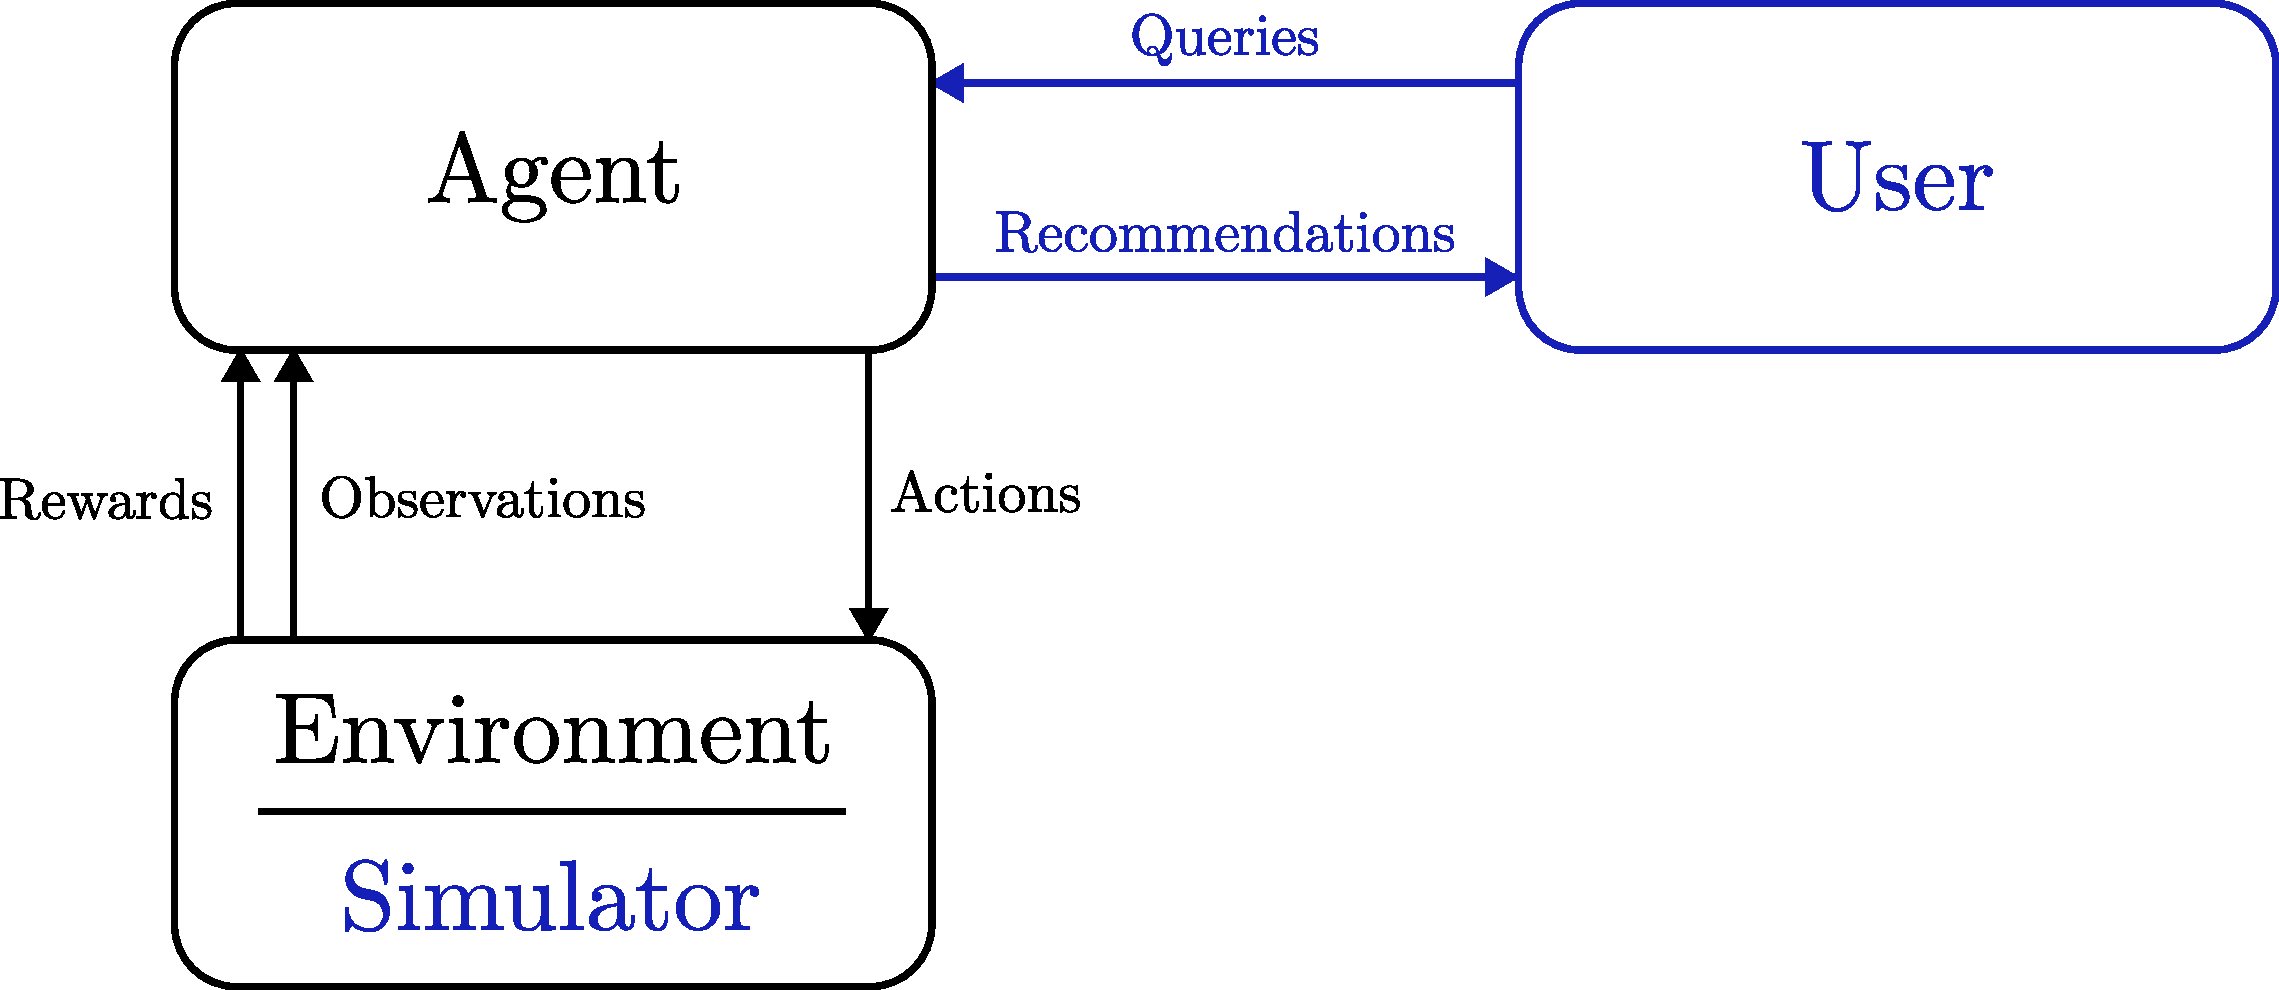
\includegraphics[width=1.0\textwidth]{figures/ch2/rl_overview.pdf} 
        \caption[An overview of reinforcement learning.]{An overview of reinforcement learning. Left: depicts the typical scenario where an agent can perform actions in an environment and is given feedback in the form of observations and rewards. Right: shows a similar scenario where the agent instead plans using a simulated environment and is then queried for recommendations about how to act in the real environment. \todo{update scale and caption for updated fig}}
        \label{fig:rl_overview}
    \end{figure}

    \hide{\todo{chatgpt the intro stuff}}

    This section serves as a brief introduction to fundamental concepts in Reinforcement Learning, and motivates . The field of Reinforcement Learning considers an agent that has to learn how to make decisions by interacting with its environment (Figure \ref{fig:rl_overview}). The agent can take actions in the environment, recieving in return \textit{observations} and \textit{rewards}, which can be used to update internal state and used to make further decisions, and the goal of the agent is to maximise the rewards that it recieves.

    Classically the agent is considered to interact with its environment directly \todo{cite sutton and barto?}, and thus must make a trade-off between exploring new strategies and exploiting learned strategies, commonly known as the \textit{exploration-exploitation trade-off}. If an agent were to try to only exploit, then it may not discover better strategies, and if an agent only explores, then it may miss out on the opportunity to exploit the best known strategy and obtain greater rewards.

    Also depicted in Figure \ref{fig:rl_overview} is a scenario where the agent is equiped with a simulator that it can use to plan and explore, and is either asked to recommend a strategy after a planning/learning phase, or is occassionally queried to recommend actions. This scenario more closely resembles how reinforcement learning is used in the modern era with greater amounts of compute power available, and interactions with the simulator occur at orders of magnitude quicker. Hence, in this scenario, the only significant real-world cost comes from following the recommendations output, to be used in the real-world environment. This changes the nature of the exploration-exploitation trade off, almost separating the two issues, where there is an emphasis on exploring during the planning phase, and the problem of providing good recommendations is concerned with pure exploitation. 

    In this thesis, the environment will always take the form of an MDP (Defintion \ref{def:mdp}), and observations will always be \textit{fully-observable}, meaning that the agent is provided with full access to the states of the MDP. Moreover, a lot of the work in this thesis concerns the simulation scenario from Figure \ref{fig:rl_overview}, and motivates our research questions around exploration: \exploreq.

    Following on from Section \ref{sec:2-1-mdps}, the remainder of this section defines \textit{value functions} and the objectives of reinforcement learning, covers \textit{Value Iteration}, a tabular dynamic programming approach to reinforcement learning, and finally Subsection \ref{sec:2-2-1-merl} covers \textit{Maximum Entropy Reinforcement Learning}.
    
    The value of a policy $\pi$ is the expected cumulative reward that will be obtained by following the policy:
    \begin{defn}
        \label{def:value}
        \label{def:q_value}
        The \textnormal{value} of a policy $\pi$ from state $s$ at time $t$ is:
        \begin{align}
            V^{\pi}(s;t) = \bb{E}_{\tau\sim\pi}\left[\sum_{i=t}^{H-1} r_t \Bigg| s_t=s \right]. \label{eq:value_fn_def}
        \end{align} 

        The \textnormal{Q-value} of a policy $\pi$, from state $s$, with action $a$, at time $t$ is:
        \begin{align}
            Q^{\pi}(s,a;t) = R(s,a) + \bb{E}_{s'\sim \suc{s}{a}} [V^{\pi}(s';t+1)]. \label{eq:q_value_fn_def}
        \end{align} 
    \end{defn}

    From the definition of the values functions the optimal value functions can be defined by taking the maximum value over all policies:
    \begin{defn}
        \label{def:optimal_value}
        \label{def:optimal_q_value}
        The \textnormal{Optimal (Q-)Value} of a state(-action pair) is defined as:
        \begin{align}
            V^*(s;t) &= \max_{\pi} V^{\pi}(s;t) \label{eq:opt_value_fn_def} \\
            Q^*(s,a;t) &= \max_{\pi} Q^{\pi}(s,a;t). \label{eq:opt_q_value_fn_def}
        \end{align}
    \end{defn}

    Value functions can also be used to define an objective function:
    \begin{defn}
        \label{def:rl_obj_fn}
        The \textnormal{(standard) reinforcement learning objective function} $J(\pi)$ is defined as:
        \begin{align}
            J(\pi) = V^{\pi}(s_0;0). \label{eq:rl_obj_fn_def}
        \end{align}

        The objective of (standard) reinforcement learning can then be stated as finding $\max_{\pi} J(\pi)$.
    \end{defn}

    The \textit{optimal policy} is the policy that maximises the objective function $J$, can be shown to be deterministic \todo{under conditions, finite?} \todo{cite}:
    \begin{defn}
        \label{def:opt_policy}
        The \textnormal{optimal (standard) policy} $\pi^*$ is the policy maximising the standard objective function:
        \begin{align}
            \pi^* = \argmax_\pi J(\pi) \label{eq:opt_policy_def}
        \end{align}
        or equivalently, the optimal standard policy can be found from the optimal Q-value function:
        \begin{align}
            \pi^*(s) = \argmax_a Q^*(s,a). \label{eq:opt_policy_from_opt_q_value}
        \end{align}
    \end{defn}

    \todo{all refs below I think can be Sutton and Barto, or [Bellman 1957] Bellman, R. 1957. Dynamic Programming. Princeton, NJ, USA: Princeton University Press, 1 edition.}

    It can be shown that the optimal (Q-)value functions satisfy the \textit{Bellman equations} \todo{refs} :
    \begin{align}
        V^*(s;t) &= \max_{a\in\cl{A}} Q^*(s,a;t), \label{eq:bellman_opt_v} \\
        Q^*(s,a;t) &= R(s,a) + \bb{E}_{s'\sim \suc{s}{a}} [V^*(s';t+1)]. \label{eq:bellman_opt_q}
    \end{align} 

    The Bellman equations admit a \textit{dynamic programming} approach which can be used to computer the optimal value functions, known as \textit{Value Iteration} \todo{ref}. In Value iteration, a table of value estimates $\hat{V}(s;t)$ are kept for each $s,t$. Given any initial estimate of the value function $\hat{V}^{0}$, the \textit{Bellman backup} operations are:
    \begin{align}
        \hat{V}^{k+1}(s;t) &= \max_{a\in\cl{A}} \hat{Q}^{k+1}(s,a;t), \label{eq:value_iter_v_backup} \\
        \hat{Q}^{k+1}(s,a;t) &= \bb{E}_{s'\sim \suc{s}{a}} [R(s,a) + \hat{V}^k(s';t+1)]. \label{eq:value_iter_q_backup}
    \end{align}

    In each iteration of Value Iteration, these values are computed for all $s\in\cl{S}$, $a\in\cl{A}$ and $t\in\{0,1,...,H\}$. The Bellman equations can be shown to be \textit{contraction operators} \todo{refs}, which can be used to show that $V^{k}\rightarrow V^*$ as $k\rightarrow \infty$, and when the state and action spaces are discrete, they will converge in a finite number of iterations. \todo{refs}









    \subsection{Maximum Entropy Reinforcement Learning}
    \label{sec:2-2-1-merl}

        In \textit{Maximum Entropy Reinforcement Learning}, the objective function is altered to include the addition of an entropy term. The addition of an entropy term is motivated by wanting to learn stochastic behaviours, that better explore large state spaces, and learn more robust behaviours under uncertainty by potentially learning multiple solutions rather than a single deterministic solution. \cite{deep_energy_policies}. 
        
        Let $\cl{H}$ denote the (Shannon) entropy function \cite{entropy}:
        \begin{align}
            \cl{H}(\pi(\cdot|s)) = \bb{E}_{a\sim\pi(\cdot|s)}[-\log \pi(a|s)] = \sum_{a\in\cl{A}} \pi(a|s) \log \pi(a|s). \label{eq:shannon_entropy_def}
        \end{align}

        In the maximum entropy objective, the relative weighting of entropy terms is included using a coefficient $\alpha$, called the \textit{temperature}. In the maximum entropy objective, analogues of the value functions can be defined, which are typically referred to as \textit{soft (Q-)values}, and similarly the maximum entropy objective is often referred to as the \textit{soft objective}.

        Soft values are defined as follows:
        \begin{defn}
            \label{def:sft_value}
            \label{def:sft_q_value}
            The \textnormal{soft value} of a policy $\pi$ from state $s$ at time $t$ is:
            \begin{align}
                V_{\sft}^{\pi}(s;t) = \bb{E}_{\tau\sim\pi}\left[\sum_{i=t}^{H-1} r_t + \alpha\cl{H}(\pi(\cdot|s_i)) \Bigg| s_t=s \right]. \label{eq:sft_value_fn_def}
            \end{align} 

            The \textnormal{soft Q-value} of a policy $\pi$, from state $s$, with action $a$, at time $t$ is:
            \begin{align}
                Q_{\sft}^{\pi}(s,a;t) = R(s,a) + \bb{E}_{s'\sim p(\cdot|s,a)} [V_{\sft}^{\pi}(s';t+1)]. \label{eq:sft_q_value_fn_def}
            \end{align} 
        \end{defn}

        Similarly, optimal soft (Q-)values can be defined by taking the maximum over policies again:
        \begin{defn}
            \label{def:optimal_sft_value}
            \label{def:optimal_sft_q_value}
            The \textnormal{Optimal soft (Q-)Value} of a state(-action pair) is defined as:
            \begin{align}
                V_{\sft}^*(s;t) &= \max_{\pi} V_{\sft}^{\pi}(s;t), \label{eq:opt_soft_value_fn_def} \\
                Q_{\sft}^*(s,a;t) &= \max_{\pi} Q_{\sft}^{\pi}(s,a;t). \label{eq:opt_soft_q_value_fn_def}
            \end{align}
        \end{defn}

        In maximum entropy reinforcement learning, the objective is to find a policy with maximal soft value:
        \begin{defn}
            \label{def:soft_rl_obj_fn}
            The \textnormal{maximum entropy (or soft) reinforcement learning objective function} $J_{\sft}(\pi)$ is defined as:
            \begin{align}
                J_{\sft}(\pi) = V_{\sft}^{\pi}(s_0;0). \label{eq:soft_rl_obj_fn_def}
            \end{align}

            The objective of maximum entropy (or soft) reinforcement learning can then be stated as finding $\max_{\pi} J_{\sft}(\pi)$.
        \end{defn}

        The optimal soft policy is defined as the policy that maximises the soft objective function $J_{\sft}$, and with knowledge of the optimal soft value and soft Q-value functions, the optimal soft policy is known:
        \begin{defn}
            \label{def:opt_sft_policy}
            The \textnormal{optimal soft policy} $\pi_{\sft}^*$ is the policy maximising the soft objective function:
            \begin{align}
                \pi_{\sft}^* = \argmax_\pi J_{\sft}(\pi). \label{eq:opt_sft_policy_def}
            \end{align}
            Given $V_{\sft}^*$ and $Q_{\sft}^*$ the optimal soft police is known to take the form \cite{deep_energy_policies}:
            \begin{align}
                \pi_{\sft}^*(a|s;t) = \exp\left(\left(Q_{\sft}^*(s,a;t) - V_{\sft}^*(s;t)\right) / \alpha \right). \label{eq:opt_sft_policy_from_opt_value_fns}
            \end{align}
        \end{defn}

        Equations similar to the Bellman equations, aptly named the \textit{Soft Bellman equations}, can be defined for maximum entropy reinforcement learning \cite{deep_energy_policies}. These equations differ to equations (\ref{eq:bellman_opt_v}) and (\ref{eq:bellman_opt_q}) by the replacement of the $\max$ operation with a \textit{softmax} or \textit{log-sum-exp} operation, and explain why the maximum entropy analogues are referred to as the \textit{soft} versions of their standard reinforcement learning counterparts.

        Similarly to standard reinforcement learning, it can be shown that the optimal soft (Q-)value functions satisfy the \textit{soft Bellman equations} \cite{deep_energy_policies}:
        \begin{align}
            V_{\sft}^*(s;t) &= \alpha \log \sum_{a\in\cl{A}} \exp\left( Q_{\sft}^*(s,a;t) / alpha \right), \label{eq:sft_bellman_opt_v} \\
            Q_{\sft}^*(s,a;t) &= R(s,a) + \bb{E}_{s'\sim \suc{s}{a}} [V_{\sft}^*(s';t+1)]. \label{eq:sft_bellman_opt_q}
        \end{align} 

        Again, similarly to standard reinforcement learning, \textit{soft Bellman backups} can be defined that admit an analogous algorithm \textit{Soft Value Iteration} \cite{deep_energy_policies}:
        \begin{align}
            \hat{V}_{\sft}^{k+1}(s;t) &= \alpha \log \sum_{a\in\cl{A}} \exp\left( \hat{Q}_{\sft}^{k+1}(s,a;t) / alpha \right), \label{eq:soft_value_iter_v_backup} \\
            \hat{Q}_{\sft}^{k+1}(s,a;t) &= R(s,a) + \bb{E}_{s'\sim \suc{s}{a}} [\hat{V}_{\sft}^k(s';t+1)]. \label{eq:soft_value_iter_v_backup}
        \end{align}














\section{Multi-Armed Bandits}
\label{sec:2-3-mab}

    \hide{\todo{Haven't started 2nd pass on this section at all, because it has the most work left to do}}

    \hide{\todo{Introduce tree search using multi-armed bandits?}}

    \hide{
    \todo{list}
    \begin{itemize}
        \item Would like to think a bit about some of the bandits work that sample actions (from adversarial I think), because they were similar to boltzmann search but I hadn't seen details about those works when writing dents
        \item Also the gradient based MAB stuff in sutton and barto book? Looks relevant? Maybe consider that as update to DENTS paper? Either way, another idea for getting good Go results.
    \end{itemize}
    }

    \todo{This section I still need to go through more finely, and add some more content}

    \todo{list}
    \begin{itemize}
        \item $R(s,a)$ is a random variable in MAB literature, but we're assuming it's a fixed value in RL
        \item Multi-Armed Bandits routines algos
        \item Exploring Bandits routines and algos
        \item Contextual Bandits routines and algos
    \end{itemize}

    \begin{figure}
        \centering
\includegraphics[width=0.5\textwidth]{figures/todo.jpg} 
        \caption[An example $K$-armed bandit problem.]{An example $K$-armed bandit problem, where \todo{description of image}}
        \label{fig:mab_example}
    \end{figure}

    \todo{Some waffel intro about this being used for decision making under uncertainty, but doesnt encorporate the sequential part of it. However, necessary for foundations, because much of sequential work builds ontop of this work}

    \todo{Also say that this can be viewed as a single state MDP with $\cl{S}=\{\bot\}$ and $\cl{A}=\{1,...,K\}$}

    \todo{Talk about relevance to sequential decision making, and tree search things, becasue they usually extend MAB algorithms}

    In the $K$-armed bandit problem, an agent is tasked with iteratively selecting one of $K$ arms, originally introduced by \todo{author} \todo{cite MAB orig}. In each iteration, once an arm is selected, say $x\in\{1,...,K\}$, and a reward $y$ is returned according to an unknown probability distribution $f_x$. Let $n$ be the number of rounds of this game that are played, and let $\mu_i=\bb{E}[y|x=i]$ be the expected reward of pulling arm $i$. 
    
    When analysing an algorithmic strategy for Multi-Armed Bandits (MABs), a quantity known as \textit{regret} is commonly used, which compares the cumulative reward obtained, compared to the maximal reward that could be obtained with full knowledge of $\{f_i\}$.

    \hide{\todo{work out how to deal with the issue of not having policies defined yet. thinhk this needs to be moved to after ch2.1}}

    \todo{some sentence}, the process of a MAB is as follows:
    \begin{itemize}
        \item for $m$ in $\{1,...,n\}$:
        \item agent selects arm $x^m$ according to policy $\pi$
        \item agent recieves reward $y^m \sim f_{x^i}$
    \end{itemize}

    \begin{defn}
        The \textnormal{(cumulative) regret} of the agent in the above process is defined as:
        \begin{align}
            \creg_{\mab}(\pi,n) = n\mu^* - \sum_{i=1}^n y^i,
        \end{align}
        where $\mu^* = max_i \mu_i$.
    \end{defn}

    To theoretically analyse algorithms for MAB problems, the quantity of expected regret, $\bb{E}[\creg_{\mab}]$ is considered. In \todo{cite} it is shown using information theory that there is a lower bound on the expected regret that an agent can achieve of $\Sigma(\log N)$, and in \todo{cite ucb} the Upper Confidence Bound (UCB) algorithm is introduced, achieving a matching upper bound of $O(\log N)$. 

    Let $N^m(j)$ be the number of times that arm $i$ has been pulled after $m$ rounds, $\bar{y}_i^m$ is the sample average of rewards recieved when pulling arm $i$: 
    \begin{align}
        \bar{y}_i^m=\frac{1}{m}\sum_{j=1}^m y^j \one[x^j=i].
    \end{align} 
    
    Then the arm selected by the UCB algorithm on the $m$th round is given by:
    \begin{align}
        \pi_{\ucb}(m) = \argmax_{j\in\{1,..,K\}} \bar{y}_j^m + b_{\ucb} \sqrt{\frac{\log(m)}{N(j)}} 
    \end{align}

    \todo{define $b_{\ucb}$}

    \todo{talk about explortaiton-exploitation trade off -- see Edwin thesis too because said it nicely}

    \todo{make sure say every arm pulled once to initialise}




    \subsection{Exploring Bandits}
    \label{sec:2-3-1-exploring-mab}

        In the pure exploration $K$-armed bandit problem \todo{cite},
        %https://link.springer.com/chapter/10.1007/978-3-642-04414-4_7#preview, 
        the game is changed slighly. The agent still gets to pull an arm each round, but after it recieves a reward each round it is given the opportunity to output a \textit{recommendation}. In exploring multi-armbed bandits (EMABs), the emphasis is now on the algorithm being able to provide the best recommendations possible, rather than trying to exploit pulling the best arm each round. In essence, this change seperates the needs to explore and exploit, the agent needs to explore with its arm pulls, and output an exploiting recommendation at the end of each round.

        \todo{some sentence}, the process of a EMAB is as follows:
        \begin{itemize}
            \item for $m$ in $\{1,...,n\}$:
            \item agent selects arm $x^m$ according to policy $\pi^m$
            \item agent recieves reward $y^m \sim f_{x^m}$
            \item agent outputs a recommendation policy $\psi^m$
        \end{itemize}

        Under this regime, the performance of an algorithm can be analysed by considering the quantity of \textit{simple regret} of the recommendation policy. The simple regret is the expected value of an \textit{instantaneous regret}, \todo{define instantaneous regret} which would come from following the recommendation policy.

        \begin{defn}
            The \textnormal{simple regret} of following the recommendation policy $\psi^m$ on the $m$th round is:
            \begin{align}
                \sreg_{\emab}(m) = \bb{E}_{i\sim\psi^m}[\mu^* - \mu_i].
            \end{align}
        \end{defn}

        \todo{talk about the bounds they show in their work}

        \todo{describe the algorithm which is pulling arms 1,2,...,K,1,2,...,K,1,..., and so on, and then recommending the arm that has the best empirical average}.



    
    \subsection{Contextual Bandits}
    \label{sec:2-3-2-contextual-mab}

        \hide{\todo{sleepy and rushed this section a bit}}

        In the contextual $K$-armed bandit problem \todo{cite}, on each round the algorithm is given a context $w\in \cl{W}$, which the algorithm does not choose. If contextual multi-armed bandit problems (CMABs), the distribution that the rewards are drawn from now depend on $w$, written $f_{w,i}$ for context $w$ for arm $i$. 

        \todo{some more words around when this is useful and why, and define CMABs}

        \todo{some sentence}, the process of a CMAB is as follows:
        \begin{itemize}
            \item for $m$ in $\{1,...,n\}$:
            \item agent recieves context $w^m$
            \item agent selects arm $x^m$ according to policy $\pi$
            \item agent recieves reward $y^m \sim f_{w^m,x^m}$
        \end{itemize}

        Similar to MABs and EMABs, the notion of regret is used to analyse CMABs. Specifically, \textit{contextual regret} is defined similarly to cumulative regret \todo{ref}, while taking into account the contexts drawn.

        \begin{defn}
            The \textnormal{(cumulative) contextual regret} of the agent in the above process is defined as:
            \begin{align}
                \ctxreg_{\cmab}(\pi,n) = \sum_{i=1}^n \mu_{w^i}^* - y^i,
            \end{align}
            where $\mu_{w}^* = \max_i \mu_{w,i}$.
        \end{defn}

        \todo{add definitions for $\mu_{w,i}$}

        \todo{Talk about contextual zooming precursor (need to read and add to litrev)}

        \todo{Write about contextual zooming, using CHMCTS paper, and use opportunity to add to litrev}
        














\section{Trial-Based Heuristic Tree Search and Monte Carlo Tree Search}
\label{sec:2-4-thts}

    \begin{figure}
        \centering
\includegraphics[width=0.5\textwidth]{figures/todo.jpg} 
        \caption[Overview of one trial of MCTS.]{Overview of one trial of MCTS, where \todo{re-describe the four stages similarly to how described inline.}}
        \label{fig:mcts}
    \end{figure}

    When considering MDPs with large state-action spaces, using tabular dynamic programming methods becomes infeasibly slow. One approach for handling large state-action spaces is to use \textit{heuristic methods}, that consider a subset of the state-action space and use of heuristic estimates for the value of states. Often these heuristic methods build a \textit{search tree} from the initial state of the MDP.

    Monte Carlo Tree Search (MCTS) refers to heuristic algorithms that build a search tree using \textit{Monte Carlo Trials}, where nodes are added to the tree based off randomly sampled trajectories. Two advantages of using MCTS methods in the modern day are: that they allow for statistical analysis, which can provide \textit{probabilistic guarantees} for the performance of the algorithm; and they offer interpretability, as the search tree can be inspected post-hoc to identify why the algorithm made certain decisions.

    MCTS trials are commonly presented using four stages, selection, expansion, simulation/heuristic and backup phases \cite{mcts_survey}, which are depicted in Figure \ref{fig:mcts}. This thesis will refer to this specific form of MCTS as \mctsone. Each of the four phases of \mctsone are described in more detail below:
    \begin{enumerate}
        \item \textit{Selection phase} - a truncated trajectory is sampled to traverse the search tree from the root node until it reaches a state not contained in the search tree;
        \item \textit{Expansion phase} - a new child node is added to the search tree;
        \item \textit{Simulation/Heuristic phase} - the new child node's value is initialised using a heuristic, often taking the form of a Monte Carlo return, obtained using a simulation with a \textit{rollout policy}; 
        \item \textit{Backup phase} - the value from the heuristic or simulation is used to backup values through the path traversed in the selection phase.
    \end{enumerate}

    Trial-Based Heuristic Tree Search (THTS) \cite{thts} generalises heuristic tree search methods used for planning, such as Trial-Based Real Time Dynamic Programming \cite{rtdp} and LAO$^*$ \cite{lao_star}. However, THTS differs slightly from how \mctsone is presented above. In a THTS trial, after the expansion/heurisitc phases are run, the trial ``switches back to the selection phase and alternate between those phases'', until the planning horizon is reached. This is similar to the trial depicted in blue in Figure \ref{fig:thts}.

    \thtspp\ewe \cite{thtspp} is introduced in Section \ref{sec:2-4-1-thts}, which is an open-source, parallelised extension of the THTS schema, and was built to facilitate the work in this thesis. Section \ref{sec:2-4-2-uct} covers the Upper Confidence Bound applied to Trees (UCT) algorithm \cite{uct,uct_long}, which is a commonly used MCTS algorithm, and Section \ref{sec:2-4-3-ments} presents the Maximum ENtropy Tree Search (MENTS) algorithm \cite{ments}, which is related to the algorithms introduced in Chapter \ref{ch:4-dents} of this thesis.
    
    


    




    \subsection{Notation}
    \label{sec:2-4-0-notation}
        To simplify notation in the presentation and analysis of \thtspp\ewe algorithms, this thesis assumes that states and state-action pairs have a one-to-one correspondance with nodes in the search tree. This assumption is purely to simplify notation for a clean presentation, and any results discussed in this thesis generalise to when this assumption does not hold. 

        Specifically, this allows the notation for value functions to avoid explicitly writing the timestep parameter, so that $V^{\pi}(s)$ can be written instead of $V^{\pi}(s;t)$.






    \subsection{Trial Based Heuristic Tree Search}
    \label{sec:2-4-1-thts}

        This subsection introduces \thtspp\ewe, which extends the Trial-Based Heuristic Tree Search (THTS) schema \cite{thts}, and aims to provide a modular library which can implement any MCTS algorithm. The changes made to the original schema allow algorithms following the four-phase \mctsone trials described previously to be encorporated. Additionally, the notion of a per-trial \textit{context} is added, which will be used in Chapters \ref{ch:5-chmcts} and \ref{ch:6-simplexmaps} for multi-objective MCTS algorithms. Additionally, beyond the scope of this thesis, contexts allow \thtspp\ewe to implement algorithms for \textit{partially-observable} environments, such as Partially Observable Monte Carlo Planning \cite{pomcp}. The remainder of this section will be presented in the context of planning for fully-observable MDPs, but generalises to partially-observable environments if \textit{observation-action histories} are used in place of states.

        In \thtspp\ewe trees consist of \textit{decision nodes} and \textit{chance nodes}. Decision nodes sample actions that can be taken by the agent, and chance nodes sample \textit{outcomes} (MDP states) that depend on the action taken and the transition function of the MDP. As such, each decision node has an associated \textit{state} and each chance node has an associated \textit{state-action pair}. Figure \ref{fig:tree_notation} shows how decision and chance nodes will be depicted in diagrams.

        \begin{figure}
            \centering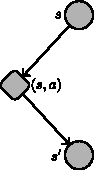
\includegraphics[width=0.2\textwidth]{figures/ch2/tree_notation.pdf} 
            \caption[Tree diagrams notation.]{Tree diagrams notation, circles will be used to denote \textit{decision nodes} that are associated with states, diamonds will be used to denote \textit{chance nodes} that are associated with state-action pairs and arrows are used to denote parent/child relationships in the tree.}
            \label{fig:tree_notation}
        \end{figure}

        A search tree $\cl{T}$ is built using Monte Carlo \textit{trials} and an overview of one trial in \thtspp\ewe is given in Figure \ref{fig:thts}. Each \thtspp\ewe trial is also split into four phases: 
        \begin{enumerate}
            \item  
                \textit{Context sampling} - a \textit{context} is sampled for the trial;
            \item 
                \textit{Selection phase} - a trajectory is sampled using a \textit{search policy}, any newly visited states (and state-action pairs) are added to $\cl{T}$ as decision nodes (and chance nodes);
            \item 
                \textit{Heuristic phase} - any new leaf nodes added in the selection phase are initialised using a \textit{heuristic function}; 
            \item 
                \textit{Backup phase} - value estimates in the search tree are updated, along the path sampled in the selection phase. 
        \end{enumerate}

        Note that the selection and expansion phases of \mctsone are encapsulated by the selection phase of \thtspp.

        \begin{figure}
            \centering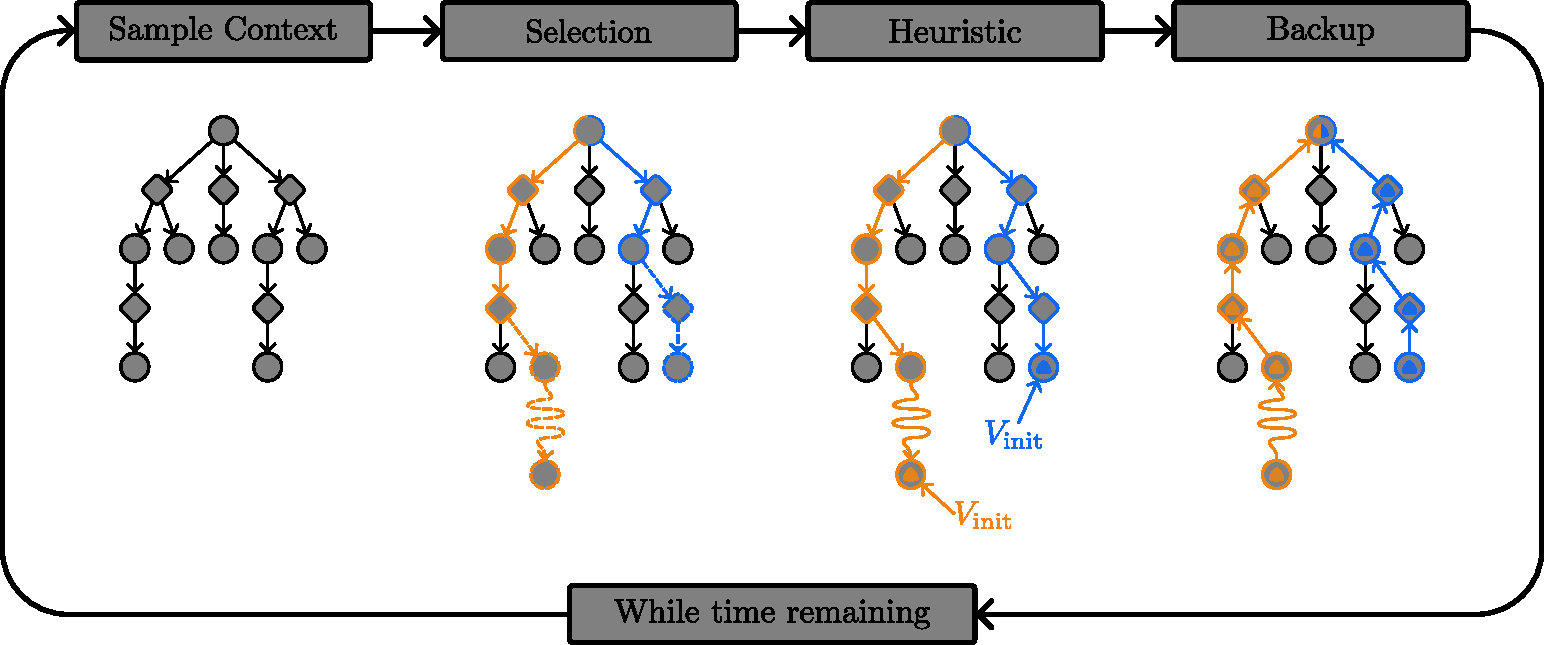
\includegraphics[width=1.0\textwidth]{figures/ch2/thts_trial.pdf} 
            \caption[Overview of one trial of \thtspp.]{Overview of one trial of \thtspp, where orange shows an example when \mctsmode\ewe is True, and blue shows an example when \mctsmode\ewe is False. From left to right: first a context is sampled, which stores any necessary per-trial state (not depicted) and the search tree at the beginning of the trial is shown; second shows the selection phase, where a trajectory is sampled and where dashed lines indicate any new nodes added; third shows that new leaf nodes are initialised using the $\Vinit$ heuristic function; and finally on the right, shows the backup phase, where the arrows directions are changed to show that information is being propogated back up the tree.}
            \label{fig:thts}
        \end{figure}

        \begin{defn}
            \label{def:search_tree}
            A \textnormal{search tree} $\cl{T}$ is a subset of the state and state-action spaces, that is $\cl{T}\subseteq \cl{S} \cup \cl{S} \times \cl{A}$, where for each $s\in\cl{T}$, there exists some truncated trajectory $\tau_{:h}$ such that $s_h = s$, each $s'\in\tau_{:h}$ is also in the tree, $s'\in\cl{T}$, and each $s',a'\in\tau{:h}$ is also in the tree, $(s',a')\in\cl{T}$.
        \end{defn}

        % \begin{defn}
        %     \label{def:cnode}
        %     \label{def:dnode}
            A \textit{decision node} refers to any state that is in the search tree: $s\in\cl{T}$. A \textit{chance node} refers to any state-action pair that is in the search tree: $(s,a)\in\cl{T}$. And a \textit{node} is used to refer to any decision or chance node in the tree. Sometimes the notation $\node(s)$ and $\node(s,a)$ will be used to make it clear that a node is being discussed, rather than a state or state-action pair.

            $N(s)$ and $N(s,a)$ denote the number of times $\node(s)$ and $\node(s,a)$ have been visited, or equivalently, the number of times $s$ and $(s,a)$ appear in trajectories sampled in \thtspp\ewe trials.

            Each decision and chance node will generally store value estimates that are algorithm dependent. $\dnodedata{s}$ is used to denote the set of values stored at node $\node(s)$, and $\cnodedata{s,a}$ for the set of value stored at node $\node(s,a)$. 

            Additionally, let $\node(s)\dotchildren$ be a mapping from actions to the chance nodes that are children of $\node(s)$. Likewise, $\node(s,a)\dotchildren$ is a mapping from outcomes to the decision nodes that are children of $\node(s,a)$.
        % \end{defn}

        \todo{make mctsmode a defn?}

        \thtspp\ewe introduces the idea of \mctsmode\ewe into the THTS schema. When running in \mctsmode, the trajectory sampled in the selection phase is truncated, and ends when the first state not in the search tree $\cl{T}$ is reached. That is, in \mctsmode, a single decision node is added to the search tree on each trial, similarly to \mctsone.  When not running in \mctsmode, the trajectory is sampled until timestep $H$, the finite horizon of the MDP, similarly to THTS. These two modes are depicted in blue (\mctsmode\ewe on) and orange (\mctsmode\ewe off) in Figure \ref{fig:thts}. 

        There are two main benefits to running an algorithm in \mctsmode. The first is that it uses significantly less memory, which can be a concern if using a large planning horizon $H$ and the tree search is going to run for a long time. The second is that if \mctsmode\ewe is used with an informative heuristic function, then it allows the algorithm to avoid wasting resouces (time and memory) on parts of the search tree that are not promising. 
        
        In contrast, when no informative heuristic is available, a random simulation is often used in \mctsone algorithms. In such cases, where memory allows, running with \mctsmode\ewe set to False can be beneficial, because states that would have been visited in the simulation phase of \mctsone are added to the tree and avoids throwing away potentially useful information.

        \todo{make context a defn?}

        \thtspp\ewe also introduces the notion of a \textit{context} that is sampled for each trial. A context is an arbitrary key-value store that is used to store any relevant data that varies from trial to trial. The context is passed to every subsequent function call in a trial of \thtspp, and can be used to store temporary state. This context will go unused for the remainder of the chapter, but will be useful in Chapters \ref{ch:5-chmcts} and \ref{ch:6-simplexmaps} when \textit{contextual tree search} is discussed. 

        To specify an algorithm in the \thtspp\ewe schema, the following need to be specified:
        \begin{description}
            \item[Value Estimates:]
                What value estimates will be stored at each decision and chance node. That is, $\dnodedata{s}$ and $\cnodedata{s,a}$ need to be defined;
            \item[Search policy:]
                A policy $\pisearch$ used to sample a trajectory for the trial, which can use values in the current search tree $\cl{T}$, and values from the heuristic action function;
            \item[Outcome Sampler:]
                A function \sampleoutcome\ewe that samples outcomes according to the environment, given a current state and action. In this thesis, this will always sample a state from the transition distribution of the MDP: $s'\sim p(\cdot|s,a)$;
            \item[Heuristic value function:]
                A function $\Vinit$ used as a heuristic to initialise values for new decision nodes added to the tree;
            \item[Heuristic action function:]
                A function $\Qinit$ used as a heuristic for Q-values when a state-action pair is not in the current search tree ;
            \item[Backup functions:]
                Two functions $\backupv$ and $\backupq$ which updates the values in decision and chance nodes respectively. These functions can use values from their children, from the sampled trajectory and from the heuristic value function;
            \item[Context sampler:]
                A function $\samplecontext$ which creates a context key-value store, and samples any initial values to be stored in the context;
            \item[MCTS mode:]
                A boolean (which will also be denoted \mctsmode) specifying if \thtspp\ewe should operate in \mctsmode. 
        \end{description}

        At the beginning of runnning a \thtspp\ewe algorithm, the search tree is initialised to $\cl{T}=\{s_0\}$. When the components detailed above are provided, the operation of a trial in \thtspp\ewe is as follows. Firstly, a context is sampled using the $\samplecontext$ function, which is available to be used by any other function in the trial. A trajectory is sampled $\tau_{:h}\sim\pisearch$ according to the search policy, which may use $\Qinit$ as necessary, and \sampleoutcome. If running in \mctsmode, then $\tau_{:h}$ is such that $s_t\in\cl{T}$ for $t=0,...,h-1$ and $s_h\not\in\cl{T}$, or $h=H$. If not running in \mctsmode, then $h=H$. The search tree is updated to include any new nodes from the sampled trajectory, $\cl{T}\leftarrow\cl{T}\cup\tau_{:h}$. The heuristic value function is used to initialise the value of the new leaf node $\dnodedata{s_h}\leftarrow \Vinit(s_h)$. Finally, for the backup phase, the $\backupq$ and $\backupv$ functions are used to update the values of $\cnodedata{s_t,a_t}$ and $\dnodedata{s_t}$ for $t=h-1,...,0$. Figure \ref{fig:thts} depicts this process, and psuedocode is given in Listing \ref{lst:thts_trial}.
        
        \begin{Listing}
            \begin{lstlisting}
def run_trial(search_tree: $\cl{T}$, 
            search_policy: $\pisearch$, 
            heuristic_fn: $\Vinit$):
    # context sampling
    cntxt = sample_context()
    # simulation phase
    $\tau_{:h}$ = sample_trajectory($\cl{T}$, $\pisearch$, cntxt)
    $\cl{T} \leftarrow \cl{T} \cup \tau_{:h}$
    # heuristic phase
    node$(s_h)$.V $\leftarrow \Vinit(s_h$, cntxt$)$
    # backup phase
    for i in $\{h-1,h-2,...,1,0\}$:
        node$(s_i,a_i)$.backup_q(node$(s_i,a_i)$.children, $\tau_{:h}$, $\Vinit(s_h)$, cntxt)
        node$(s_i)$.backup_v(node$(s_i)$.children, $\tau_{:h}$, $\Vinit(s_h)$, cntxt)

def sample_trajectory(search_tree: $\cl{T}$, 
                    search_policy: $\pisearch$, 
                    cntxt):
    i = 0
    while (not mcts_mode or $s_{\texttt{i}}\in\cl{T}$) and i < H:
        $a_{\texttt{i}} \sim \pisearch(\cdot | s_{\texttt{i}},$ cntxt$)$ 
        $r_{\texttt{i}} \leftarrow R(s_{\texttt{i}}, a_{\texttt{i}})$
        $s_{\texttt{i+1}} \leftarrow$ sample_outcome$(s_{\texttt{i}}$, $a_{\texttt{i}}$, cntxt$)$
        i += 1
    return $(s_0,a_0,r_0,s_1,...,s_{\texttt{i-1}}, a_{\texttt{i-1}},r_{\texttt{i-1}}, s_{\texttt{i}})$

def sample_outcome($s$, $a$, cntxt):
    $s' \sim p(\cdot | s, a)$
    return $s'$
            \end{lstlisting}
            \caption[Psuedocode for running a trial in \thtspp.]{Psuedocode for running a trial in \thtspp.}
            \label{lst:thts_trial}
        \end{Listing}


    



    
    \subsection{Upper Confidence Bounds Applied to Trees (UCT)}
    \label{sec:2-4-2-uct}

        Upper Confidence Bounds Applied to Trees (UCT) \cite{uct,uct_long} is a commonly used tree search algorithm, which is based on the Upper Confidence Bounds (UCB) \todo{cite} algorithm covered in Section \todo{ref}. UCT can be viewed as running UCB on a non-stationary MAB at every decision node, where it is non-stationary because the rewards obtained depend on the decisions that children nodes made. The remainder of this subsection will outline how UCT can be defined using the the \thtspp schema given in Section \ref{sec:2-4-1-thts}.

        In UCT \mctsmode\ewe is set to True. And at each decision and node of UCT a sample average $\Vuct$ and $\Quct$ is used for a value estimate. The search policy that UCT then follows is given by:
        \begin{align}
            \piuct(s) = \argmax_{a\in\cl{A}} \Quct(s,a) + b_{\uct} \sqrt{\frac{\log(N(s))}{N(s,a)}}, \label{eq:uct_policy}
        \end{align}
        where $b_{\uct}$ is a \textit{bias} parameter that controls the amount of exploration UCT will perform. In Equation (\ref{eq:uct_policy}), when $N(s,a)=0$ there is a division by zero, which is taken as $\inf$, and ties are broken uniformly randomly. Note that like UCB (Section \todo{ref}), this results in every action being taken once to obtain an initial value estimate, and as such, setting $\Qinit$ is unnecessary for UCT.   
        
        There are two common approaches to implementing $\Vinit$ in UCT: the first consisting of using a function approximation $\tilde{V}$ and setting $\Vinit=\tilde{V}$ \todo{cite some papers doing this, rave?}, where $\hat{V}$ aims to approximate the optimal value function $V^*$; the second approach consists of using a \textit{rollout policy} \todo{cite some papers doing this}. When a rollout policy $\pirollout$ is used, a Monte Carlo estimate $\hat{V}^{\pirollout}$ is used to estimate the value function $V^{\pirollout}$ and is used for $\Vinit$.

        Let $\tau_{:h}\sim\piuct$, be the trajectory sampled in the selection phase of UCT, meaning that a decision node for $s_h$ is added to the search tree, and needs to be initialised with $\Vinit$. When using a rollout policy, the truncated trial is completed using the rollout policy $\tau_{h:H}\sim\pirollout$ to provide the Monte Carlo estimate at $s_h$:
        \begin{align}
            \hat{V}^{\pirollout}(s_h) = \sum_{i=h}^{H-1} r_i. \label{eq:rollout_value_estimate}
        \end{align}

        If no informative policy is available to be used for $\pirollout$, then uniformly random policy is often used \todo{cite}.

        In UCT the backups $\backupv$ and $\backupq$ update the (sample average) value estimates. Letting heuristic value for the leaf node be $\tilde{r} = \Vinit(s_h)$, they are computed as follows:
        \begin{align}
            \Quct(s_t,a_t) &\leftarrow 
                \frac{1}{N(s_t,a_t)} \left( (N(s_t,a_t)-1) \Quct(s_t,a_t) 
                    + \tilde{r} + \sum_{i=t}^{h-1} r_i \right) \label{eq:uct_backup_q} \\
            \Vuct(s_t) &\leftarrow 
                \frac{1}{N(s_t)} \left( (N(s_t)-1) \Vuct(s_t,a_t) 
                    + \tilde{r} + \sum_{i=t}^{h-1} r_i \right) \label{eq:uct_backup_v}
        \end{align}  

        \todo{Make a comment about how when use a random rollout, that using mctsmode OFF is identical?}








    \subsection{Maximum Entropy Tree Search}
    \label{sec:2-4-3-ments}

        Maximum ENtropy Tree Search (MENTS) \cite{ments}, in contrast to UCT, focuses on the maximum-entropy objective, and uses soft Bellman backups (Equations \todo{ref}) to update its value estimates. In its original presentation \mctsmode\ewe is set to True, and it uses the soft value estimates $\Vments$ and $\Qments$. The MENTS search policy is given by:
        \begin{align}
            \piments(a|s) &= 
                (1-\lambda_s)\exp\left(\frac{1}{\alpha_{\ments}}\left(\Qments(s,a)-\Vments(s)\right)\right) 
                    + \frac{\lambda_s}{|\cl{A}|}, \label{eq:ments_policy}
        \end{align}
        where $\lambda_s=\min(1,\epsilon/\log(e+N(s))),$ with $\epsilon \in (0,\infty)$ is an exploration parameter, and $\alpha_{\ments}$ is the temperature paramter used in MENTS for the maximum entropy objective (the coefficient of the entropy term in Equation (\todo{ref})).

        In MENTS the backups $\backupv$ and $\backupq$ update the soft value estimates and are updated using soft Bellman backups as follows:
        \begin{align}
            \Qments(s_t,a_t) &\leftarrow 
                R(s_t,a_t) + \sum_{s'\in\suc{s}{a}} \left( \frac{N(s')}{N(s_t,a_t)} \Vments(s') \right), \label{eq:ments_backup_q} \\
            \Vments(s_t) &\leftarrow 
                \alpha \log \sum_{a\in\cl{A}} \exp \left(\frac{1}{\alpha}\Qments(s_t,a) \right). \label{eq:ments_backup_v} 
        \end{align}

        In \cite{ments}, the heuristic value function left as an arbitrary evaluation function, but is set using a function approximation $\Vinit=\tilde{V}$ in experiments. The heuristic action function is set to zero, $\Qinit(s,a)=0$, but they also suggest that if \textit{policy network} $\tilde{\pi}$ is available, then the heuristic action function can alternatively be set to $\Qinit(s,a)=\log \tilde{\pi}(s|a)$. 















\section{Multi-Objective Reinforcement Learning}
\label{sec:2-5-morl}

    \hide{\todo{Rushing through the todo's here so probably needs another round for 2nd pass, not doing any adding labels to defs and equations, not making any diagrams}}

    \hide{\todo{This section defo want a fair bit more work. First read through the MORL survey paper, add to index, and then go through and rewrite a bunch of things}}

    \hide{\todo{Define an interface for pareto front and convex hull objects}}
    \hide{\todo{Follow https://arxiv.org/abs/2103.09568 more closely, and write a bit more waffel in this section}}

    \todo{Link back to some of the multi objective questions}

    This thesis follows a utility based approach to Multi-Objective Reinforcement learning similar to \todo{cite}. For a full review of Multi-Objective Reinforcement Learning see \todo{cite}. This work will specifically consider \textit{linear utility} functions and the \textit{decision support scenario} (Figure \ref{fig:mo_decision_support}), which will be defined more precisely below.

    \begin{figure}
        \centering
\includegraphics[width=0.5\textwidth]{figures/todo.jpg} 
        \caption{The decision-support scenario for Multi-Objective Reinforcement Learning.]{The decision-support scenario for Multi-Objective Reinforcement Learning.}}
        \label{fig:mo_decision_support}
    \end{figure}

    This section defines the multi-objective conterparts to various definitions in Section \ref{sec:2-1-mdps} and \ref{sec:2-2-rl}. Outside of this section, the prefix ``multi-objective'' may be dropped where it should be clear from context, however bold typeface will consistently be used to denote any vector variables or functions.

    To specify problems with multiple objectives, the reward function of an MDP changed to give a vector of rewards, rather than a scalar reward:
    \begin{defn}
        \label{def:mo_mdp}
        A \textnormal{Multi-Objective Markov Decision Process} (MOMDP) is a tuple $\bfcl{M}=(\cl{S},s_0,\cl{A},\bff{R},p,H)$, where $\cl{S}$ is a set of states, $s_0\in\cl{S}$ is an initial state, $\cl{A}$ is a set of actions, $\bff{R}(s,a)$ is a vector reward function $\cl{S}\times \cl{A}\rightarrow \bb{R}^D$, where $D$ is the dimension of the rewards and the MOMDP, $p(s' | s,a)$ is a next state transition distribution $\cl{S} \times \cl{A} \times \cl{S} \rightarrow [0,1]$ and $H\in\bb{N}$ is a finite-horizon time bound.
    \end{defn}

    Now multi-objective trajectories are defined:
    \begin{defn}
        \label{def:mo_trajectory}
        A \textnormal{multi-objective trajectory} $\tau$, is a sequence of state, action and vector rewards, that is induced by a policy $\pi$ and MOMDP $\bfcl{M}$ pair. Let the trajectory be $\bff{\tau} = (s_0, a_0, \bff{r}_0, s_1, a_1, \bff{r}_1, ..., s_{H-1}, a_{H-1}, \bff{r}_{H-1}, s_H)$, where $a_t \sim \pi(\cdot|s_t)$, $\bff{r}_t=\bff{R}(s_t,a_t)$ and $s_{t+1} \sim \suc{s_t}{a_t}$. 
        
        The notations used for single-objective trajectories (Definition \ref{def:trajectory}) will also be used for multi-objective trajectories too. Such as, $\bff{\tau}\sim\pi$ for sampling trajectories using policies, and $\bff{\tau}_{i:j}$ for truncated trajectories.
    \end{defn}

    Similarly, multi-objective variants of the (Q-)value of a policy are defined:    
    \begin{defn}
        \label{def:mo_value}
        \label{def:mo_q_value}
        The \textnormal{multi-objective value} of a policy $\pi$ from state $s$ at time $t$ is:
        \begin{align}
            \bff{V}^{\pi}(s;t) = \bb{E}_{\bff{\tau}\sim\pi}\left[\sum_{i=t}^{H-1} \bff{r}_t \Bigg| s_t=s \right].
        \end{align} 

        The \textnormal{multi-objective Q-value} of a policy $\pi$, from state $s$, with action $a$, at time $t$ is:
        \begin{align}
            \bff{Q}^{\pi}(s,a;t) = R(s,a) + \bb{E}_{s'\sim \suc{s}{a}} [\bff{V}^{\pi}(s';t+1)].
        \end{align} 
    \end{defn}

    In the corresponding point of the single-objective reinforcement learning section (Section \ref{sec:2-2-rl}), the the optimal (Q-)value functions and the objective of single-objective reinforcement learning were defined. However, in a multi-objective setting there is no longer a \textit{total ordering} over values, and so there maybe be multiple vectors that could be ``optimal''. To resolve this issue, a \textit{utility function} or \textit{scalarisation function} is used to map multi-objective values to scalars.

    \begin{defn}
        \label{def:simplex}
        \label{def:weight}
        \label{def:context}
        The \textnormal{($D$-dimensional) Simplex} consists of the set of $D$-dimensional vectors, whose entries are non-negative and sum to one. More formally, the $D$ dimensional simplex is $\Delta^D = \{\bff{w}\in\bb{R}^D|w_i > 0, \sum_i w_i = 1\}$.

        The elements of the $D$-dimensional Simplex will be referred to as \textnormal{weight vectors} in this thesis, as they will be used to specify preferences over the $D$ dimensions of the reward function.
    \end{defn}

    \begin{defn}
        \label{def:utility_fn}
        \label{def:scalarisation_fn}
        A \textnormal{utility function} (or \textnormal{scalarisation function}) $u:\mathbb{R}^D\times\Delta^D \rightarrow \bb{R}$ is used to map from a multi-objective value $\bff{v}\in\bb{R}^D$ and a weighting over the objectives $\bff{w}\in\Delta^D$ to a scalar value. That is, according to the utility function $u(\cdot;\bff{w})$ the multi-objective value $\bff{v}$ is mapped to the scalar value $u(\bff{v};\bff{w})$.
    \end{defn}

    Of particular interest in this thesis is the \textit{linear utility function} where the scalar value takes the form of a dot-product:
    \begin{defn}
        \label{def:linear_utility_fn}
        \label{def:linear_scalarisation_fn}
        The \textnormal{linear utility function} $u_{\lin}$ is the utility function defined by:
        \begin{align}
            u_{\lin}(\bff{v};\bff{w}) = \bff{w}^\top \bff{v}.
        \end{align}
    \end{defn}

    Equiped with a scalarisation function and a weight vector any set of multi-objective values can be ordered, which allows sets of \textit{possibly optimal} policies to be defined. Letting $\Pi$ be the set of all possible policies, sets of solution policies can be defined:
    \begin{defn}
        \label{def:undominated_set}
        \label{def:convex_hull}
        The \textnormal{undominated set} of policies $U(\Pi;u)\subseteq\Pi$, with respect to a utility function $u$,  is the set of policies for which there is a weight vector $\bff{w}\in\Delta^D$ where the scalarised value is maximised: 
        \begin{align}
            U(\Pi;u) = \left\{\pi\in\Pi\ \big|\ \exists \bff{w}\in\Delta^D. \forall \pi'\in\Pi: u(\bff{V}^{\pi}(s_0;0);\bff{w}) \geq u(\bff{V}^{\pi'}(s_0;0);\bff{w}) \right\}.
        \end{align}

        In particular, the \textnormal{convex hull} of policies $CH(\Pi)$ is the undominated set with respect to the linear utility function $u_{\lin}$. That is $CH(\Pi)=U(\Pi;u_{\lin})$.
    \end{defn}    

    Undominated sets often have an infinite cardinality, and as such are infeasibil to compute. However, in undominated sets there are often many reduntant policies that obtain the same scalarised values. Instead of computing an undominated set, it is more feasible to compute a \textit{coverage sets} which contain at least one policy that maximises the scalarised value given any weight vector $\bff{w}$:
    \begin{defn}
        \label{def:coverage_set}
        \label{def:convex_coverage_set}
        A set $CS(\Pi;u)\subseteq U(\Pi)$, is a \textnormal{coverage set} with respect to a utility function $u$, if for every weight vector $\bff{w}\in\Delta^D$, there is a policy $\pi\in CS(\Pi;u)$ that maximises the value of $u(\cdot;\bff{w})$. That is, for $CS(\Pi;u)$ to be a coverage set, the following statement must be true:
        \begin{align}
            \forall \bff{w}\in\Delta^D. \exists \pi\in CS(\Pi;u). \forall \pi'\in\Pi: u(\bff{V}^{\pi}(s_0;0);\bff{w}) \geq u(\bff{V}^{\pi'}(s_0;0);\bff{w}).
        \end{align}

        Again, in particular, any set $CCS(\Pi)$ is a \textnormal{convex coverage set} if it is a coverage set with respect to the linear utility function $u_{\lin}$. 
    \end{defn}

    To compute a coverage set, it is often useful to first compute the multi-objective values that could be obtained, and then later use the data structures used by the algorithm to read out the selected policy. 

    \begin{defn}
        \label{def:mo_value_set}
        The \textnormal{(multi-objective) value set} with respect to a set of policies $\Pi'\subseteq\Pi$ is defined as:
        \begin{align}
            \valset(\Pi') = \{\bff{V}^{\pi}(s_0;0) | \pi \in \Pi'\}.
        \end{align}
    \end{defn}

    Because this thesis considers the decision support scenario, the objective of an multi-objective algorithm will be to compute a $\valset(CCS(\Pi))$, however, coverage sets are not unique. In the case of the linear utility function, multi-objective values that obtain the same scalarised value will lie on a hyperplane (see Figure \todo{ref}). As a result, the vectors in $\valset(CCS(\Pi))$ will geometrically form a \textit{(parital) convex hull} (also see Figure \ref{fig:convex_hull_geometry}). Given this, it is most common to compute the multi-objective values that lie at the vertices of the geometric convex hull (also see Figure \ref{fig:convex_hull_geometry}). 

    For the remainder of this thesis, the primary objective of multi-objective algorithms will be to compute the value set $\valset(CCS(\Pi))$ that lies at the vertices of the geometric convex hull, which will be referred to as the \textit{Convex Hull Value Set} (CHVS). \todo{make this a defn, going to use the acronym a lot}

    \begin{figure}
        \centering
\includegraphics[width=0.5\textwidth]{figures/todo.jpg} 
        \caption[The geometry of Convex Coverage Sets.]{The geometry of Convex Coverage Sets, shown with $D=2$. In all images, the points depicted correspond to a value set $\valset(\Pi)$. Left: demonstrates that values obtaining the same scalarised value, for a linear utility function with weight vector $\bff{w}$, lie on a hyperplane with a normal vector of $\bff{w}$. Right: depicts a (geometric) partial convex hull. Any set of vectors $\bfcl{V}\subseteq\valset(\Pi)$ that contains a point touching each edge of the geometric convex hull is a valid (value set of a) convex coverage set, and the points that are filled denotes one of such sets. Finally, the circles, which are at  the extreme points of the geometric convex hull mark the (value set of the) convex coverage set that is typically computed.}
        \label{fig:convex_hull_geometry}
    \end{figure}

    \hide{
        \todo{
            Here are some things that wrote at the end when icky and ill. Also editing this section tired, so maybe consider adding them into the above on another pass, or moving into ch3, or maybe we covered them and just delete:

            Should acknowledge some things. Often we actually compute the value set of a convex coverage set. Often we compute a very specific convex coverage set, which is the extreme points of the convex hull. Also that the term convex hull is typically used to refer to any of the previous three sets (value set, convex coverage set, convex hull). And finally, say that often with methods that compute the value set can often use tagging to compute the policies after the fact, and cite some of the pomdp algorithms from LPK that actually explain the tagging

            Additionally, this thesis focusses on the decision support scenario as outlined in (TODO: cite), with a linear utility function. In the decision support scenario the true weight vector is unknown, and so the objective is to compute a convex coverage set. When a convex coverage set is produced, it is then provided to a user that picks their most preferred policy or value from the coverage set. After this policy is selected, it can be used as a single solution to the problem that the user was trying to solve. 
        
            Moreover, in the case of MCTS algorithms, by having the user select a preferred policy, it implicitly forces the user to chose a preference over the objectives, as the policy corresponds to a weight vector that it is optimal for. As MCTS algorithms are often used in an online fashion, where planning is interleaved with execution, this implicitly selected weight can be used for any online execution needed, effectively reducing the multi-objective problem into a single-objective problem. 
        }
    }




    \subsection{Convex Hull Value Iteration}
    \label{sec:2-5-1-chvi}

        Convex Hull Value Iteration (CHVI) \cite{chvi} is a tabular dynamic programming algorithm similar to Value Iteration \todo{ref}. In CHVI the value functions of value iterations are replaced by sets of vectors, which are estimates of the convex hull value set.

        CHVI maintains estimates of CHVS's at each state $\Vchvi(s;t)$.

        One important operation for CHVI is \cprune, which returns that undominated set of vectors from a given set of vectors $\bfcl{V}$:
        \begin{align}
            \cprune(\bfcl{V}) = \{\bff{v}\in\bfcl{V} | \exists \bff{w}\in\Delta^D. \forall \bff{v}'\in\bfcl{V}-\{\bff{v}\}. \bff{w}^\top \bff{v} > \bff{w}^\top \bff{v}' \}.
        \end{align}

        The \cprune\ewe operation can be implemented using \textit{linear programming} \todo{cite}, and an example of its operation on a set of vectors is given in Figure \ref{fig:convex_prune}.

        \begin{figure}
            \centering
\includegraphics[width=0.5\textwidth]{figures/todo.jpg} 
            \caption[An example of the \cprune\ewe operation.]{An example of the \cprune\ewe operation. The circles and triangles form a vector set $\bfcl{V}$, and the circles denote the set $\cprune(\bfcl{V})$.}
            \label{fig:convex_prune}
        \end{figure}

        Additionally, to define a multi-objective version of value iteration, an arithmetic over sets of vectors needs to be defined. An example of the following arithmetic is given in Figure \ref{fig:vectorset_arithmetic} Given the sets of vectors $\bfcl{U}$ and $\bfcl{V}$, define multiplication by a scalar $s$, addition with a vector $\bff{x}$ and addition between sets as follows:
        \begin{align}
            \bff{x} + s\bfcl{V} &= \{\bff{x} + s\bff{v} | \bff{v}\in\bfcl{V} \} \\
            \bfcl{U} + \bfcl{V} &= \{ \bff{u}+\bff{v} | \bff{u}\in\bfcl{U}, \bff{v}\in\bfcl{V} \}.
        \end{align}

        \begin{figure}
            \centering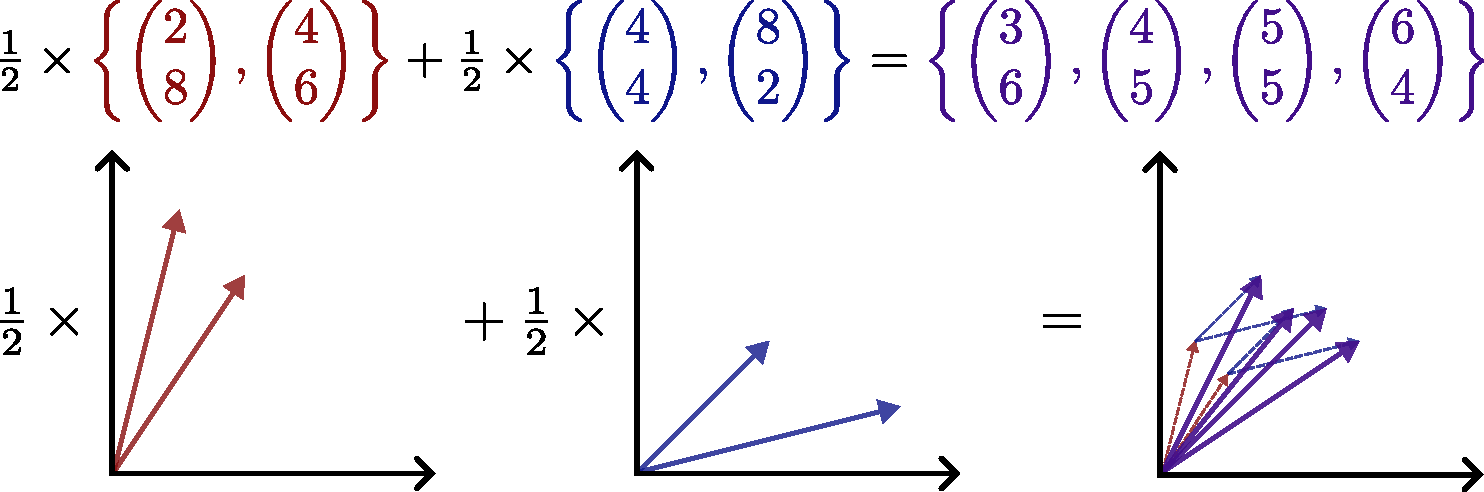
\includegraphics[width=1.0\textwidth]{figures/ch2/ch_arithmetic.pdf} 
            \caption[An example of arithmetic over sets of vectors.]{An example of arithmetic over sets of vectors, where \todo{describe specifics more specifically, and note that addition by a vector is not shown here, but is similar. Also something looks a bit off about the purple vectors, maybe want to add a light grid behind the graphs? Just to give perspective. Reference that this demonstrates the scalar multiplication from equation (xxx) and addition between sets in equation (xxx). And yes, want the grid, but do later}.}
            \label{fig:vectorset_arithmetic}
        \end{figure}

        Now to define the multi-objective Bellman backups used in CHVI, let $\hat{\bfcl{V}}^0(s) = \{ \bff{0} \}$, where $\bff{0}=(0,...,0)\in\bb{R}^D$. The CHVI backups are then:
        \begin{align}
            \Vchvi^{k+1}(s;t) &= \cprune \left( \bigcup_{a\in\cl{A}} \Qchvi^{k+1}(s,a;t) \right), \\
            \Qchvi^{k+1}(s,a;t) &= \bb{E}_{s'\sim \suc{s}{a}} [\bff{R}(s,a) + \Vchvi^k(s';t+1)].
        \end{align}
        
        This again parallels the Bellman backups use in single-objective value iteration \todo{ref}, where the max operation is replaced by the \cprune\ewe operation over the set of achievable values from the current state $s$: $\bigcup_{a\in\cl{A}} \Qchvi^{k+1}(s,a;t)$.

        Extracting actions and policies from the computed CHVSs is not explicitly discussed in \cite{chvi}. However, vectors can be \textit{tagged} with actions which allows for a policy to be read out after selecting a value in a CHVS. Consider \todo{having a CHVS for V and Q, set Qtagged to Q with the action in the Q function, and then say that V is computed same as equation XXX, and for convex prune, if there is (v,a) and (v,a'), then break ties randomly. An example of using this tagging to read out policies is given in Figure} \ref{fig:chvs_tagging}.
        
        \todo{some hidden stuff here to consider?}
        \hide{
            However,CHVI is very similar to the \textit{witness algorithm} for Partially Observable MDPs \todo{cite lpk paper}, where it is 
            
            To read out policies from the computed convex hull value sets, vectors can be \textit{tagged} with actions, similar to work in partially observable MDPs \todo{cite lpk paper}. For an example of this, see Figure \ref{fig:chvs_tagging}.
        }

        \begin{figure}
            \centering
\includegraphics[width=0.5\textwidth]{figures/todo.jpg} 
            \caption[An example of using tagging with convex hull value sets.]{An example of using tagging with convex hull value sets. An MOMDP is shown, with its associated CHVS's. \todo{colour code the tagging and use arrows to show two different policies being read out from the initial state, and write the corresponding description here}.}
            \label{fig:chvs_tagging}
        \end{figure}

        \todo{talk about the POMDP action tagging things}












\section{Sampling From Catagorical Distributions}
\label{sec:2-6-sampling}

    \hide{\todo{Rushing through the todo's here so probably needs another round for 2nd pass, not doing any adding labels to defs and equations, not making any diagrams}}

    \hide{\todo{Reference to chapter (TODO: ref ch:4-dents) section where talk about using this with THTS}}

    \hide{\todo{clean this up generally, wrote it in a rush. Also trying not to use notation that I may want to use later. Would like }}

    \todo{still need to do another pass through this}

    \todo{this section needs figs still}

    Much of the work in this thesis will involve sampling from catagorical distributions. Let $f:\{1,...,m\}\rightarrow\bb{R}$ be the probability mass function of a catagorical distribution with $m$ categories. Suppose that we want to sample $i\sim f$. A naive method to sample from $f$ will take $O(m)$ time, where a value is sampled from $\textnormal{Uniform}(0,1)$ is often used as follows:

    \begin{lstlisting}
def sample_catagorical($f$):
    threshold $\sim \textnormal{Uniform}(0,1)$
    i = 0
    accumulated_mass = 0
    while (accumulated_mass < threshold):
        i += 1
        accumulated_mass += $f($i$)$
    return i
    \end{lstlisting}
    \todo{add label and caption for listing}
    % TODO: make a figure env for code

    However, the \textit{Alias method} \todo{cite1, cite2} can instead be used, with $O(m)$ preprocessing time to construct an \textit{Alias table}, and can sample from $f$ in $O(1)$ time. In Figure \todo{ref} we provide an example of an alias table. A value can be sampled using the alias table by sampling two random numbers, one from $\textnormal{Uniform}(\{1,...,m\})$ and one from $\textnormal{Uniform}(0,1)$. To sample from the alias table, one of the entries is sampled uniformly randomly using the sample from $\textnormal{Uniform}(\{1,...,m\})$, each entry in the table contains three values, \texttt{threshold}, \texttt{cat\_one} and \texttt{cat\_two}, from which if we let $a\sim\textnormal{Uniform}(0,1)$, we would then return \texttt{cat\_one} if $a<$\texttt{threshold} and \texttt{cat\_two} otherwise. Psuedocode for this is as follows:

    \begin{lstlisting}
def sample_from_alias_table(alias_table):
    index $\sim \textnormal{Uniform}(\{1,...,m\})$
    cat_one, cat_two, threshold = alias_table[index]
    a $\sim \textnormal{Uniform}(0,1)$
    if (a < threshold):
        return cat_one 
    return cat_two
    \end{lstlisting}
    \todo{add label and caption for listing}

    In \todo{cite} it is shown \todo{double check that it's proven} that an alias table can be constructed from an arbitrary probability mass function for a catagorical distribution, such that the probability of sampling any catagory from the alias table is identical to the probability of sampling it from the original probability mass function. 
    
    \todo{add fig, and in caption verify that the example alias table maintains the correct masses for each category}

    Following \todo{cite}, we can construct an alias table as follows:

    \begin{lstlisting}
def build_alias_table($f$):
    pass
    \end{lstlisting}
    \todo{add label and caption for listing}

    \todo{write the build alias table psuedocode (use wiki it was good)}










    
    








\hide{
    \todo{after finished chapter, make sure no errors from latex}

    \todo{after finished chapter, make sure all equations labelled}

    \todo{after finished chapter, make sure all sections correctly referenced, changed sec:2-5-sampling to sec:2-4-sampling, removed the sec:2-4-momcts, added sec:2-5-mabs}

    \todo{after finished chapter, make sure all abbreviations and accronyms added and correct}
}